% ============================================================
%  SECTION 1: What is an exchange rate?          (Member 1)
% ============================================================
\section{What is an exchange rate?}

Chai in Chennai is paid for in rupees, but coffee in New York needs US dollars and a meal in Dubai needs dirhams. So whenever goods, services or savings cross a border, one currency has to be swapped for another. The price of that swap is the \keyterm{exchange rate}{The price of one currency in terms of another, for example ₹95 per US dollar.}: the price of one currency in terms of another (National Council of Educational Research and Training [NCERT], 2007). In India it is set mainly by buyers and sellers in a market, and like the price of onions it can change from minute to minute.

Indian banks write the rate as a \keyterm{direct quote}{The price of one unit of foreign currency in home currency, e.g.\ US\$1 = ₹95.}, ``US\$1 = ₹95'', which is the number of rupees needed to buy one dollar (Jayadev, 2021). Flip it and you get the \keyterm{indirect quote}{How much foreign currency one unit of home currency buys, e.g.\ ₹1 = US\$0.0105.}, ``₹1 = US\$0.0105'', which is the number of dollars one rupee buys. This chapter always uses the direct quote, rupees per dollar (₹/\$), so a bigger number means a weaker rupee. At ₹95 instead of ₹88, every rupee buys fewer dollars \seesec{Appreciation and depreciation: who wins, who loses?}.

\begin{figure}[htbp]
  \centering
  \begin{minipage}[c]{0.40\linewidth}
    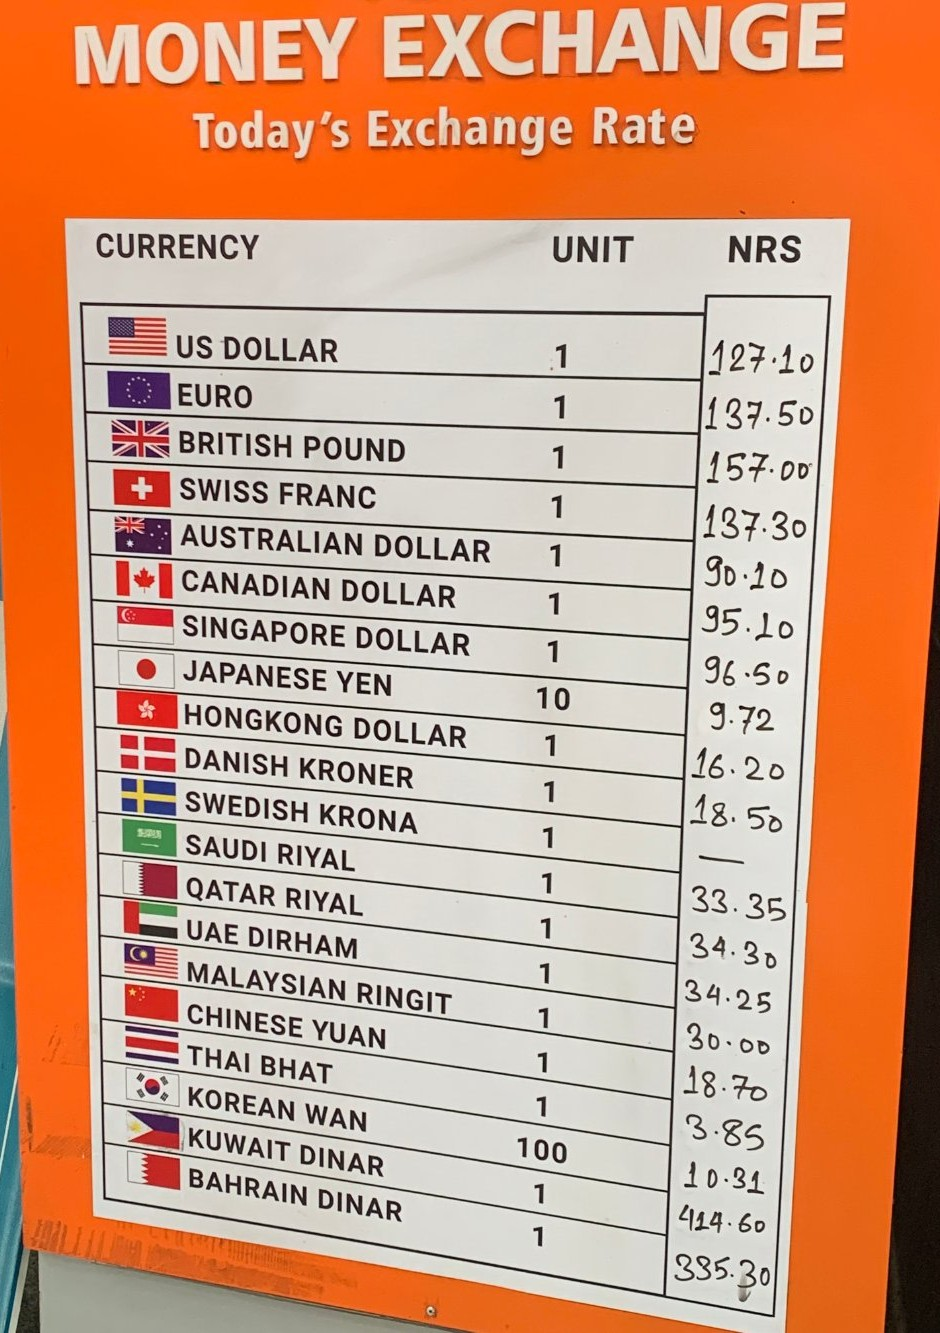
\includegraphics[width=\linewidth]{images/kathmandu_board.jpg}
  \end{minipage}\hfill
  \begin{minipage}[c]{0.56\linewidth}
    \caption{A money exchange board at Kathmandu airport, January 2023.}
    \label{fig:m1-board}
    \small\sffamily
    Each row is a \emph{direct quote}: the price of one unit of a foreign currency in Nepalese rupees (NRs). A US dollar costs NRs~127.10 and a UAE dirham, the currency Ravi earns, about NRs~34. The Japanese yen is priced per 10 yen, because a single yen is worth very little.
    \figsource{Photograph by Chainwit. (2023), \href{https://commons.wikimedia.org/wiki/File:Arrival_at_Kathmandu_Tribhuvan_Airport_(01-2023)_-_img_06.jpg}{Wikimedia Commons}, \href{https://creativecommons.org/licenses/by/4.0/}{CC BY 4.0}, cropped.}
  \end{minipage}
\end{figure}

\begin{didyouknow}{Every board hides two prices}
Banks and money changers quote two rates for each currency: a lower rate at which they buy it from you and a higher rate at which they sell it to you. Suppose a bank buys dollars at ₹93.50 and sells them at ₹96.50. Change ₹10,000 into dollars and you get US\$103.63. Change them straight back and you get only ₹9,689. The missing ₹311 is the bank's earning, called the \textbf{spread}. Spreads are usually widest for cash at airport counters, which is why travellers lose the most there.
\figsource{The rates in this example are hypothetical.}
\end{didyouknow}

\subsection{Why everyone watches the dollar}
Why does the news talk only about the rupee's price in dollars? Because the dollar is the world's working currency. In April 2025 it was on one side of 89 per cent of all currency trades (Bank for International Settlements [BIS], 2025). Crude oil, India's biggest import, is priced in dollars, and only about 6 per cent of India's exports are invoiced in rupees (Reserve Bank of India [RBI], 2026a). Since July 2022 the RBI has allowed Indian firms to settle foreign trade in rupees (RBI, 2022), but most still choose the dollar, because almost everyone, everywhere, will accept it.

The dollar even reaches currencies that seem unrelated. The UAE dirham, which Ravi earns, has been fixed at 3.6725 dirhams per US dollar since 1997 (Nagraj, 2024). So when a dollar costs more rupees, so does a dirham, and every dirham Ravi sends home turns into more rupees.
